\clearpage
\subsection{premi/client}
\begin{figure}[H]
\begin{center}
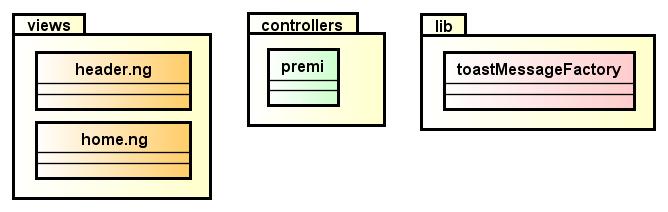
\includegraphics[scale=0.50]{img/diapkg/client.png}
\caption{Diagramma del package premi/client}
\end{center}
\end{figure}


%-------  diagramma di un template %
\subsubsection{premi/client/views/header.ng}

\begin{description}
%-------  descrizione del template%
\item[Descrizione] \hfill
	Template che genera un header per la pagina principale dell'applicazione
	\item[Note] \hfill
	\begin{itemize}
			\item Deve mostrare il nome dell'utente, se loggato, oppure un pulsante per loggarsi
			\item Deve mostrare un pulsante per accedere alla pagina di modifica della passsword, se l'utente è loggato
	\end{itemize}
\end{description}

%-------  diagramma di un template %
\subsubsection{premi/client/views/home.ng}

\begin{description}
%-------  descrizione del template%
\item[Descrizione] \hfill
	Template della pagina principale dell'applicazione
	\item[Note] \hfill
	\begin{itemize}
			\item Deve mostrare il logo dell'applicazione
			\item Deve mostrare un pulsante per registarsi, se l'utente non è loggato
	\end{itemize}
\end{description}

%-------  diagramma di un template %
\subsubsection{premi/client/controllers/premi}

\begin{description}
%-------  descrizione del template%
\item[Descrizione] \hfill
	Controller della pagina principale dell'applicazione. Rende \textit{currentUser} "reattivo", ossia utilizza il metodo getReactively di urigo:angular-meteor$_G$ per fare in modo che venga inviato un segnale ogni volta che currentUser cambia
\end{description}

%-------  diagramma di un template %
\subsubsection{premi/client/lib/toastMessageFactory}

\begin{description}
%-------  descrizione del template%
\item[Descrizione] \hfill
	Semplice factory che restituisce una funzione per l'invio di notifiche o messaggi di errore all'utente. Sfrutta il metodo \texttt{Materialize.toast()} del framework$_G$ Materialize$_G$.
%-------  lista delle classi associate%	
\item[Dipendenze] \hfill
	\begin{itemize}
		\item \textbf{Materialize}: (dipendenza non dichiarata esplicitamente) il framework Materialize viene utilizzato richiamare il suo metodo \texttt{Materialize.toast()}, reso disponibile a livello globale dopo l'avvio del server.
	\end{itemize}
\end{description}

